\documentclass[border=4pt,dvisvgm]{standalone}
\usepackage{tikz}
\usetikzlibrary{arrows.meta,positioning,shapes.geometric,fit,calc,backgrounds}
\begin{document}
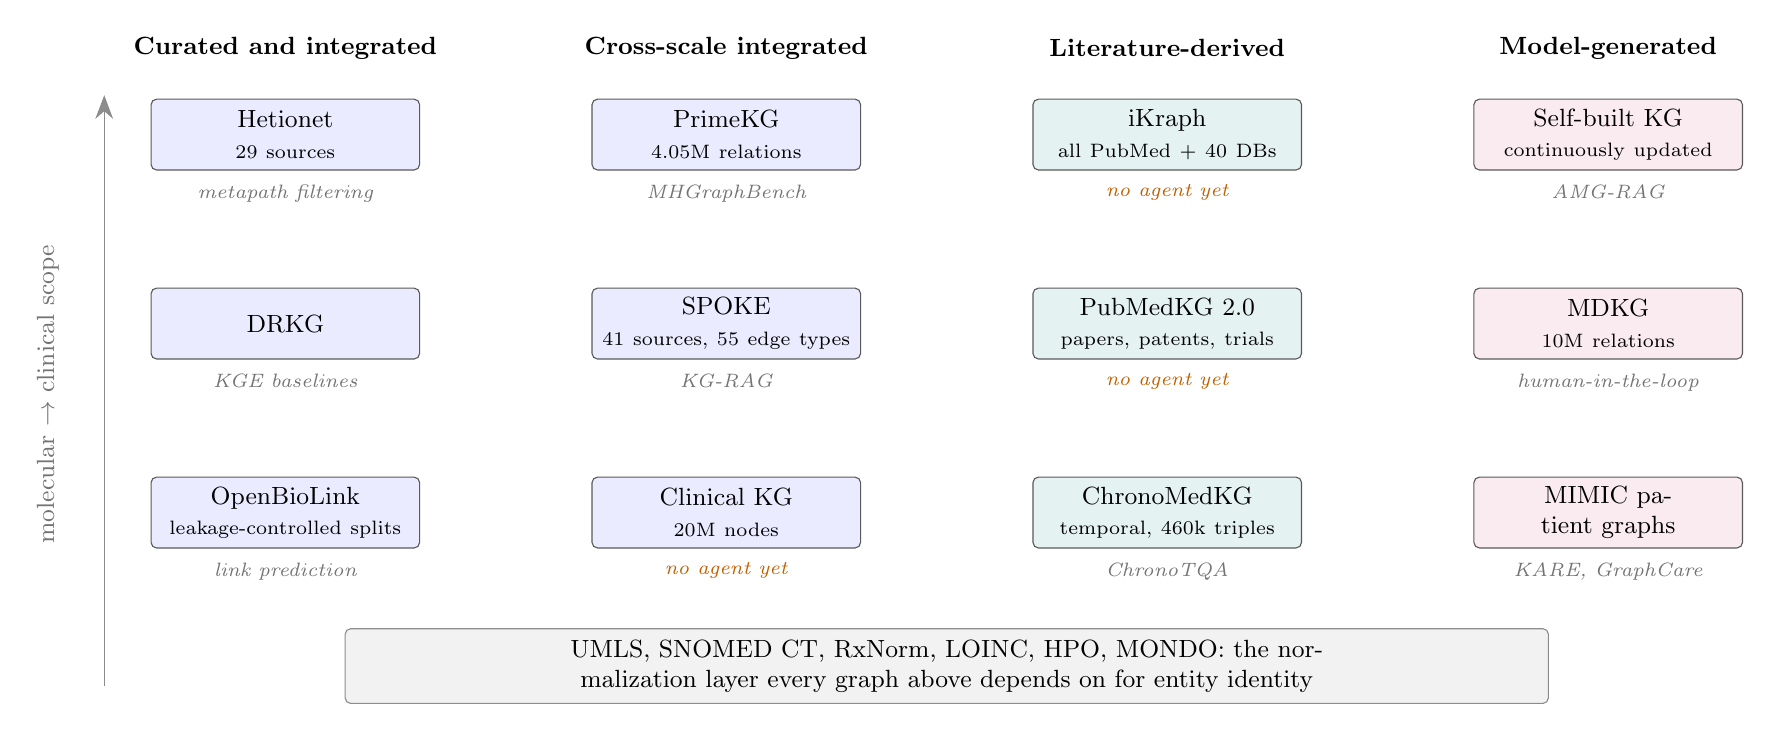
\begin{tikzpicture}[
  font=\small,
  g/.style={draw=black!65, rounded corners=2pt, align=center, inner sep=3pt,
            text width=32mm, minimum height=9mm},
  curated/.style={g, fill=blue!8},
  litder/.style={g, fill=teal!10},
  gen/.style={g, fill=purple!8},
  onto/.style={draw=black!45, rounded corners=2pt, fill=black!5, align=center,
               inner sep=4pt, text width=150mm},
  sys/.style={font=\scriptsize\itshape, text=black!55, align=center, text width=32mm},
  gap/.style={font=\scriptsize\itshape, text=orange!75!black, align=center, text width=32mm},
  axis/.style={draw=black!45, -{Stealth[length=3mm]}}
]

% column headers
\node[font=\small\bfseries] at (0,1.5)    {Curated and integrated};
\node[font=\small\bfseries] at (5.6,1.5)  {Cross-scale integrated};
\node[font=\small\bfseries] at (11.2,1.5) {Literature-derived};
\node[font=\small\bfseries] at (16.8,1.5) {Model-generated};

% scope axis
\draw[axis] (-2.3,-6.6) -- (-2.3,0.9);
\node[rotate=90, anchor=south, font=\small, text=black!55] at (-2.75,-2.9) {molecular $\rightarrow$ clinical scope};

% ---- curated
\node[curated] (hetio) at (0,0.4)   {Hetionet\\{\scriptsize 29 sources}};
\node[sys, below=0.6mm of hetio] {metapath filtering};
\node[curated] (drkg) at (0,-2.0)   {DRKG};
\node[sys, below=0.6mm of drkg] {KGE baselines};
\node[curated] (obl) at (0,-4.4)    {OpenBioLink\\{\scriptsize leakage-controlled splits}};
\node[sys, below=0.6mm of obl] {link prediction};

% ---- cross-scale
\node[curated] (primekg) at (5.6,0.4) {PrimeKG\\{\scriptsize 4.05M relations}};
\node[sys, below=0.6mm of primekg] {MHGraphBench};
\node[curated] (spoke) at (5.6,-2.0)  {SPOKE\\{\scriptsize 41 sources, 55 edge types}};
\node[sys, below=0.6mm of spoke] {KG-RAG};
\node[curated] (ckg) at (5.6,-4.4)    {Clinical KG\\{\scriptsize 20M nodes}};
\node[gap, below=0.6mm of ckg] {no agent yet};

% ---- literature-derived
\node[litder] (ikraph) at (11.2,0.4) {iKraph\\{\scriptsize all PubMed + 40 DBs}};
\node[gap, below=0.6mm of ikraph] {no agent yet};
\node[litder] (pkg) at (11.2,-2.0)   {PubMedKG 2.0\\{\scriptsize papers, patents, trials}};
\node[gap, below=0.6mm of pkg] {no agent yet};
\node[litder] (chrono) at (11.2,-4.4) {ChronoMedKG\\{\scriptsize temporal, 460k triples}};
\node[sys, below=0.6mm of chrono] {ChronoTQA};

% ---- model-generated
\node[gen] (amg) at (16.8,0.4)   {Self-built KG\\{\scriptsize continuously updated}};
\node[sys, below=0.6mm of amg] {AMG-RAG};
\node[gen] (mdkg) at (16.8,-2.0) {MDKG\\{\scriptsize 10M relations}};
\node[sys, below=0.6mm of mdkg] {human-in-the-loop};
\node[gen] (mimic) at (16.8,-4.4) {MIMIC patient graphs};
\node[sys, below=0.6mm of mimic] {KARE, GraphCare};

% ---- terminology band
\node[onto] at (8.4,-6.35) {UMLS, SNOMED CT, RxNorm, LOINC, HPO, MONDO: the normalization layer every graph above depends on for entity identity};
\end{tikzpicture}%
\end{document}
